\documentclass[11pt]{article}

\usepackage[margin=1in]{geometry}
\usepackage{amsmath,amssymb}
\usepackage{booktabs}
\usepackage{tabularx}
\usepackage{array}
\usepackage{xcolor}
\usepackage{graphicx}
\usepackage{float}
\usepackage{microtype}
\usepackage{hyperref}

\newcolumntype{Y}{>{\raggedright\arraybackslash}X}
\newcolumntype{L}[1]{>{\raggedright\arraybackslash}p{#1}}

\hypersetup{
  colorlinks=true,
  linkcolor=blue!45!black,
  citecolor=blue!45!black,
  urlcolor=blue!45!black
}

\newcommand{\fresh}{\texttt{fresh\_adaptive}}
\newcommand{\frozen}{\texttt{continuation\_frozen\_greedy}}
\newcommand{\adaptive}{\texttt{continuation\_adaptive}}
\newcommand{\qqprofit}{0.320496}
\newcommand{\qqprice}{1.784199}

% Filled from analysis/deng_frozen_mature_dqn_100k after the confirmatory bundle.
\newcommand{\frozenprofit}{0.300520}
\newcommand{\jointprofit}{0.288464}
\newcommand{\designpremium}{+0.012055}
\newcommand{\designcilow}{-0.013116}
\newcommand{\designcihigh}{+0.039539}
\newcommand{\adaptivechange}{-0.043904}
\newcommand{\adaptivecilow}{-0.068590}
\newcommand{\adaptivecihigh}{-0.021540}
\newcommand{\adaptivepvalue}{0.001953}
\newcommand{\frozenadvantage}{+0.065779}
\newcommand{\frozenadvlow}{+0.037465}
\newcommand{\frozenadvhigh}{+0.094129}
\newcommand{\frozenadvp}{0.021484}
\newcommand{\adaptiveadvantage}{+0.007274}
\newcommand{\adaptiveadvlow}{-0.006799}
\newcommand{\adaptiveadvhigh}{+0.022045}
\newcommand{\adaptiveadvp}{0.753906}
\newcommand{\advantagechange}{-0.058504}
\newcommand{\advchangelow}{-0.090627}
\newcommand{\advchangehigh}{-0.030138}
\newcommand{\advchangep}{0.021484}

\title{Frozen-Opponent Evaluation and Live-Update Continuation in Algorithmic Pricing}
\author{Danila Malafeev\thanks{Replication code and seed-level data: \url{https://github.com/danilamalafeev/algorithmic-pricing-continuation}}\\
National Research University Higher School of Economics\\
\texttt{dsmalafeev@edu.hse.ru}}
\date{June 24, 2026}

\begin{document}
\maketitle

\begin{abstract}
Holding a pricing rival fixed and allowing it to continue updating define
different evaluation objects. We study this distinction in a Calvano-style
Bertrand-logit duopoly. A DQN entrant is trained against ten independently
trained mature Q-learning incumbents, with three DQN initializations per
incumbent. After training, the same entrant--incumbent pair is evaluated with
the incumbent either frozen or permitted to resume Q-updates. The entrant
profit advantage is positive in 9 of 10 frozen-checkpoint means but only 6 of
10 live-update means; entrant own profit falls in all 10 matched comparisons.
Separately, six configured learners spanning public reward feedback,
known-payoff counterfactuals, Q-supervised auxiliary objectives, and direct
Q-update-model access remain below the ten-seed mature Q-vs-Q reference in
mean own profit and mean market price. These finite-budget results show that
evaluation protocol is part of the estimand and that the tested richer
configurations do not reproduce the Q-vs-Q high-price convention. Lower
logged prices raise model-implied consumer surplus; total-welfare conclusions
depend on the learner and on a binned-trajectory approximation.
\end{abstract}

\noindent\textbf{Keywords:} algorithmic pricing; reinforcement learning;
industrial organization; multi-agent evaluation; Bertrand competition.

\section{Introduction}

Algorithmic-pricing experiments often hold one agent fixed while another
learns. This measures entrant performance against a fixed pricing rule, not
performance when the rival's update rule remains active. The distinction
matters when the incumbent is a mature tabular Q-learner: its recurrent-path
behavior may be stable even though much of its off-path Q-table reflects
seed-specific learning history.

This paper asks two questions. \textbf{RQ1} asks how post-training entrant
performance changes when a mature incumbent is frozen versus permitted to
resume Q-updates. \textbf{RQ2} asks whether the high-price convention produced by mature
Q-vs-Q self-play is readily recovered by richer representation learning,
counterfactual payoff feedback, or escalating access to incumbent
information---from public observation through Q-supervised training targets
to direct Q-table and update-rule access.

The first question revisits a specific experimental design in Shidi Deng,
Schiffer, and Bichler~\cite{shidideng2025}. Their heterogeneous-agent experiment
pretrains TQL in self-play for one million steps, freezes it, and trains a new
DQN or PPO entrant for 100,000 steps. We reproduce the economic logic of that
design across ten independently trained mature incumbents and explicitly
separate frozen evaluation from live-update-permitted continuation. The second
question is motivated by Ai Deng's distinction between algorithmic collusion
and algorithmic confusion~\cite{aideng2026}: a high-price outcome can reflect
limited exploration or counterfactual reasoning rather than superior strategic
intelligence.

Two findings organize the paper. First, frozen-opponent performance varies
substantially across mature Q-tables, and allowing incumbent Q-updates changes
the entrant's measured profit. Second, DQN, full-information regret matching,
a JEPA-style latent-prediction DQN, and a Q-supervised opponent-model DQN
remain below the mature Q-vs-Q reference. A Q-row reconstruction DQN and a
model-based Q-update rollout planner also remain below it, but are reported
separately because their training or planning uses incumbent-Q information.

\section{Related Work}

Calvano et al.~\cite{calvano2020} show that independent tabular Q-learners can
produce supracompetitive prices in a Bertrand-logit environment. Subsequent
work questions whether such outcomes reflect strategic coordination, limited
exploration, synchronized design, or algorithmic misspecification
\cite{abada2024,carissimo2025}. Ai Deng~\cite{aideng2026} synthesizes this
literature as a distinction between high-price outcomes and the mechanisms
that generate them.

Shidi Deng et al.~\cite{shidideng2025} extend the pricing comparison to DQN and
PPO. Their homogeneous DRL agents generally price below TQL, while a new DRL
agent earns high profit against a pretrained TQL agent that no longer updates.
Our RQ1 concerns the interpretation of that latter protocol, not the paper's
broader comparison of algorithm classes.

In MARL, an opponent's learning creates nonstationarity
\cite{hernandez2017,papoudakis2019}. Opponent-shaping methods make this
dependence explicit~\cite{foerster2018,fung2024}. We apply the same distinction
to pricing: fixed-opponent performance and performance with a live update rule
are different estimands.

\section{Model and Design}

\subsection{Bertrand-Logit Game}

The stochastic game is
\[
\mathcal G=\langle \{O,V\},\mathcal S,\{\mathcal A_i\}_{i\in\{O,V\}},
P,\{\pi_i\}_{i\in\{O,V\}},\delta\rangle .
\]
Each firm chooses one of \(K=15\) prices. With continuous symmetric Nash and
joint-monopoly prices \(p^N\) and \(p^M\), the grid is
\[
\underline p=p^N-\xi(p^M-p^N),\qquad
\overline p=p^M+\xi(p^M-p^N),
\]
\[
p(a)=\underline p+\frac{a}{K-1}(\overline p-\underline p),
\qquad a\in\{0,\ldots,K-1\}.
\]
The baseline uses \(c_i=1\), \(q_i=2\), outside quality \(q_0=0\), market mass
\(D=1\), logit scale \(\mu=0.25\), and \(\xi=0.1\). These values imply
\(p^N\approx1.473\) and \(p^M\approx1.925\).

Demand share and stage profit are
\[
\rho_i(p_i,p_{-i})=
\frac{\exp((q_i-p_i)/\mu)}
{\exp(q_0/\mu)+\sum_{j\in\{O,V\}}\exp((q_j-p_j)/\mu)},
\]
\[
\pi_i(a_O,a_V)=
\bigl(p(a_i)-c_i\bigr)D
\rho_i\bigl(p(a_i),p(a_{-i})\bigr).
\]
The public state is the previous joint action,
\(s_t=(a^O_{t-1},a^V_{t-1})\), so \(|\mathcal S|=225\).

\subsection{Incumbent Learning}

The incumbent updates by off-policy Q-learning:
\[
Q_V(s_t,a^V_t)\leftarrow Q_V(s_t,a^V_t)+
\alpha\left[
r^V_t+\delta\max_{a'}Q_V(s_{t+1},a')-Q_V(s_t,a^V_t)
\right],
\]
where \(\alpha=0.15\) and \(\delta=0.95\). Its exploration schedule is
\[
\varepsilon_t=\exp(-4\times10^{-6}t).
\]
At ten million steps, \(\varepsilon_{10M}=\exp(-40)\approx4.25\times10^{-18}\).
Thus a mature incumbent is behaviorally deterministic absent an injected
shock. ``Adaptive continuation'' means that Q-updates are permitted; it does
not imply substantial exploration or a greedy-policy switch in every window.

\subsection{Evaluation Protocols}

\begin{table}[H]
\centering
\caption{Evaluation protocols and estimands.}
\label{tab:protocols}
\small
\begin{tabularx}{\textwidth}{lccY}
\toprule
Protocol & Start & Incumbent rule & Measured object \\
\midrule
\fresh & New run & Q-learning & Joint learning from a fresh initialization \\
\frozen & Matched trained pair & Greedy; \(Q,t\) fixed & Performance against a fixed pricing rule \\
\adaptive & Matched trained pair & Greedy plus Q-update & Sensitivity to post-training update permission \\
\bottomrule
\end{tabularx}
\end{table}

For RQ1, each of ten independently trained 10M Q-vs-Q checkpoints is frozen
while three DQN entrants learn for 100,000 steps. DQN hyperparameters through
step 100,000 match the registered joint-learning control, including a 50,000
step exploration decay. The post-training evaluation is:
\begin{enumerate}
\item clone the same trained DQN and mature-incumbent checkpoint into both
branches and warm the public history from the saved joint state;
\item hold DQN weights, replay memory, target network, and optimizer fixed;
choose DQN actions greedily, with its recurrent reservoir reset identically;
\item in \frozen{}, choose the incumbent action greedily and hold its Q-table
and learning clock fixed;
\item in \adaptive{}, use the incumbent's saved exploration clock and apply
its Q-learning update after every realized transition;
\item run 3,000 evaluation periods in each of 64 vectorized rollout streams
under matched branch seeds, then average prices and profits over 192,000
observations.
\end{enumerate}
At 10M steps the incumbent's exploration probability is approximately
\(4.25\times10^{-18}\), so the branch contrast is primarily update permission,
not injected exploratory action. The mature checkpoint is the statistical
unit; the three DQN initializations are averaged within checkpoint.

For RQ2, each learner configuration is evaluated from its own-run final checkpoint and
compared with the distribution of ten independently trained mature Q-vs-Q
checkpoints. Vectorized environments are rollout batches, not replications.
Exact two-sample permutation tests use the learner seed and mature-checkpoint
seed as the units and test equality of the two distributions under
exchangeability. Percentile bootstrap intervals use 10,000 independent
resamples of both groups. Holm adjustment is applied across all six tested
configurations, separately for profit and mean market price.

\section{Results}

\subsection{Reference Distribution}

The ten mature Q-vs-Q checkpoints have mean own profit
\(\bar\pi^{QQ}=\qqprofit\) (SD \(0.008366\)) and mean market price
\(\bar p^{QQ}=\qqprice\) (SD \(0.043988\)). The distribution, rather than a
single canonical checkpoint, is the reference for inference. It is
environment- and implementation-specific.

\subsection{RQ1: Frozen-Opponent Performance and Update Permission}

Under frozen evaluation, the DQN entrant's profit exceeds incumbent profit by
\frozenadvantage{} on average, with checkpoint bootstrap 95\% CI
\([\frozenadvlow,\frozenadvhigh]\). The difference is positive in 9 of 10
checkpoint means (exact two-sided binomial sign test \(p=\frozenadvp\)).
Under live-update-permitted continuation, the entrant gap is
\adaptiveadvantage{} (95\% CI \([\adaptiveadvlow,\adaptiveadvhigh]\);
\(6/10\) positive; sign-test \(p=\adaptiveadvp\)). Relative to frozen
evaluation, the gap changes by
\advantagechange{} (95\% CI \([\advchangelow,\advchangehigh]\);
the change is negative in \(9/10\) checkpoints; sign-test
\(p=\advchangep\)). This is a protocol-sensitivity exercise motivated by
experiments in which a new DRL agent is trained against a pretrained TQL
incumbent; it is not an exact replication of any one prior implementation.

As a secondary design comparison, mean DQN own profit is \frozenprofit{} under
frozen mature entry and \jointprofit{} at the registered 100k checkpoint of
joint learning from scratch. The difference is \designpremium{} (hierarchical
percentile-bootstrap 95\% CI \([\designcilow,\designcihigh]\)). This descriptive
contrast has no permutation \(p\)-value because the two designs have different
sampling structures and combines incumbent maturity with freezing. Holding
the trained DQN and starting checkpoint fixed, permission to update changes
DQN own profit by \adaptivechange{} on average (95\% CI
\([\adaptivecilow,\adaptivecihigh]\)); the change is negative in all ten
checkpoint means (sign-test \(p=\adaptivepvalue\)).
Figure~\ref{fig:protocol-result} shows the two principal contrasts.

\begin{figure}[H]
\centering
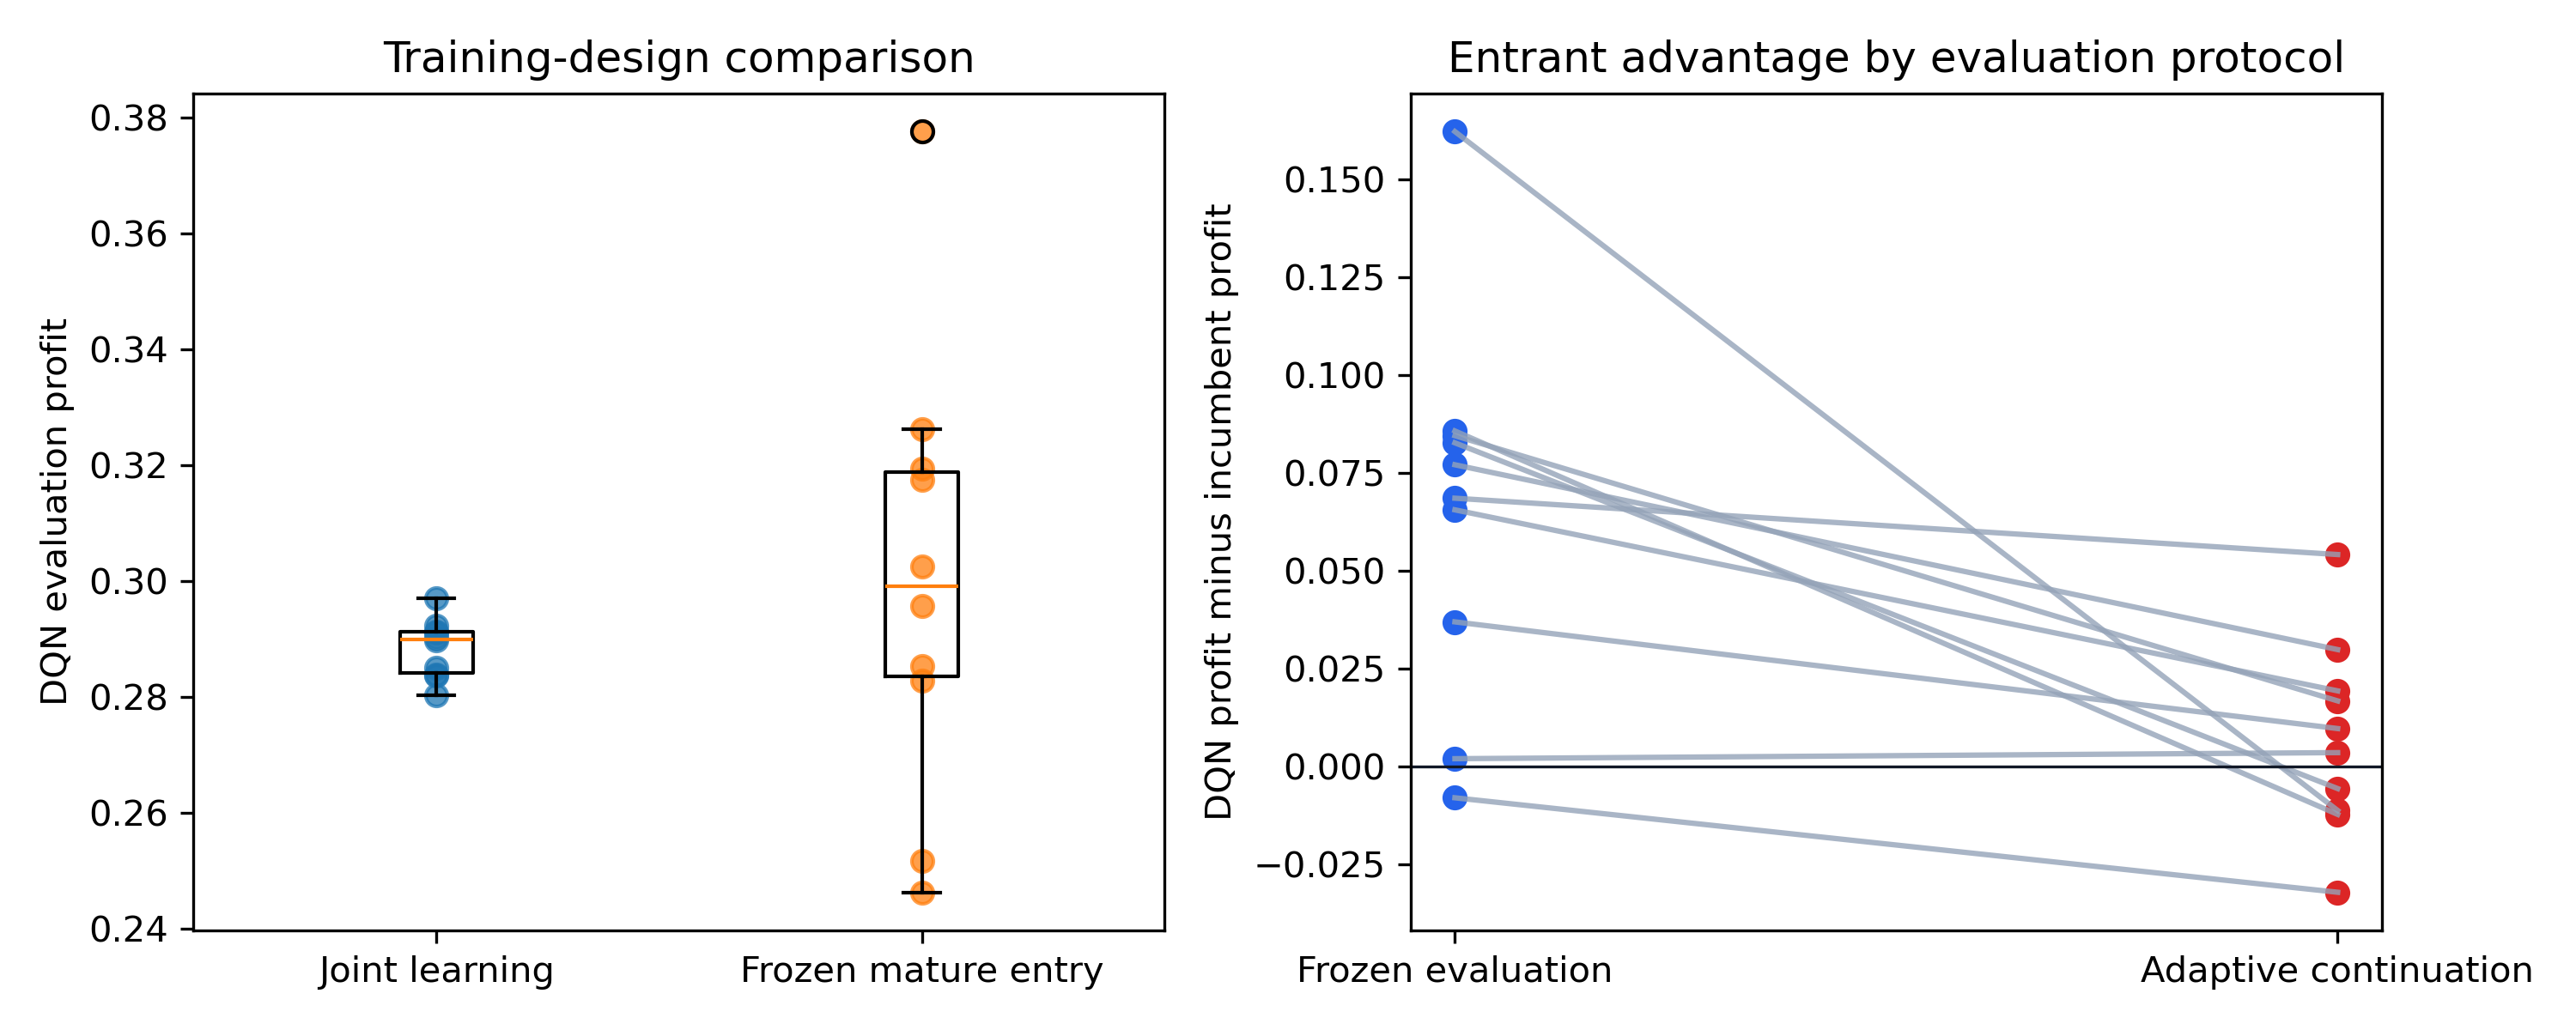
\includegraphics[width=0.92\textwidth]
{../analysis/deng_frozen_mature_dqn_100k/deng_design_contrast.png}
\caption{DQN own profit across training designs (left) and entrant-minus-
incumbent profit under matched evaluation protocols (right). Points in the
right panel are mature-checkpoint means over three DQN seeds.}
\label{fig:protocol-result}
\end{figure}

The protocol result is therefore narrower than ``DQN beats TQL.'' A tested DQN
can earn substantially more than a fixed mature incumbent, but the magnitude
is checkpoint-specific and changes when the same incumbent is permitted to
update.

\subsection{RQ2: Learner Configurations}

\begin{table}[H]
\centering
\caption{Final own profit and market price by tested learner.}
\label{tab:architectures}
\small
\begin{tabular}{lllrrr}
\toprule
Access layer & Learner & Horizon & Seeds & Own profit & Mean price \\
\midrule
Public reward & DQN & 1M & 10 & 0.287577 & 1.682100 \\
Known model & Full-information regret matching & 1M & 10 & 0.268153 & 1.555464 \\
Public reward & Latent-prediction DQN & 100k & 10 & 0.292334 & 1.595135 \\
Q-supervised & Opponent-model DQN & 100k & 10 & 0.289470 & 1.634459 \\
\midrule
Q-supervised & Q-row reconstruction DQN & 100k & 10 & 0.280474 & 1.642845 \\
Model access & Q-update rollout planner, \(H=5\) & 150k & 10 & 0.295937 & 1.665133 \\
\midrule
Reference & Mature Q-vs-Q & 10M & 10 & \qqprofit & \qqprice \\
\bottomrule
\end{tabular}
\end{table}

All tested rows lie below the mature Q-vs-Q mean in both own profit and mean
market price, at training budgets from 100k to 1M steps against the 10M mature
reference. Exact permutation tests and bootstrap intervals are reported in
Appendix~\ref{app:statistics}. The evidence tests recoverability of the
high-price convention along the information ladder; it does not rank
configurations, whose horizons and objectives differ.

\begin{table}[H]
\centering
\caption{Information and feedback used by each configured learner.}
\label{tab:information}
\scriptsize
\begin{tabularx}{\textwidth}{L{0.24\textwidth}L{0.15\textwidth}YL{0.15\textwidth}L{0.11\textwidth}}
\toprule
Learner & Runtime state & Learning signal & Direct model access & Evaluation \\
\midrule
DQN & Public & Realized reward & None & Live update \\
Full-information regret matching & Public & Counterfactual payoffs for all own actions & Known payoff model & Live update \\
Latent-prediction DQN & Public & Reward plus next-latent target & None & Live update \\
Q-supervised opponent-model DQN & Public & Reward plus incumbent-Q labels & None at action time & Live update \\
Q-row reconstruction DQN & Public & Reward plus normalized incumbent Q-row & None at action time & Live update \\
Q-update rollout planner & Public & Simulated rollout value & Incumbent Q-table and update rule & Default final \\
\bottomrule
\end{tabularx}
\end{table}

Table~\ref{tab:information} orders the configurations along an escalating
information ladder: public reward, known counterfactual payoffs, richer latent
representations, incumbent-Q-derived training targets, and---at the top---direct
Q-table and update-rule access. The Q-supervised rows act from public features
but use incumbent-Q labels in training; the rollout planner simulates the
incumbent table and update rule directly. Read as one stress test, the result is
uniform: no rung of the ladder recovers the high-price convention, including the
two privileged configurations that observe or simulate the incumbent's
Q-structure.

\subsection{Model-Implied Welfare}

For each logged training interval \(b\), consumer surplus is approximated by
\[
 \widehat{CS}_{b}=D\mu\log\left[
\exp(q_0/\mu)+\sum_{i\in\{O,V\}}\exp((q_i-p_i)/\mu)
\right],
\]
where \(p_i\) is the mean posted price recorded for that interval. Interval
total welfare is
\[
\widehat{TW}_{b}=\widehat{CS}_{b}
+\overline{\pi}_{O,b}+\overline{\pi}_{V,b}.
\]
The last 100,000 training steps are averaged with weights equal to interval
length. DQN and full-information regret matching use twenty 5,000-step bins;
the other learners use one hundred 1,000-step bins. The reference is computed
for each of the ten mature Q-vs-Q final-policy evaluations and then averaged.

\begin{table}[H]
\centering
\caption{Last-100k log-bin welfare approximation relative to the mature
Q-vs-Q final-policy reference. Intervals are seed-bootstrap 95\% CIs for the
mean difference.}
\label{tab:binned-welfare}
\scriptsize
\begin{tabular}{lrrr}
\toprule
Learner & \(\Delta CS\) & \(\Delta\) joint profit & \(\Delta TW\) [95\% CI] \\
\midrule
DQN & +0.086178 & -0.056022 & +0.030157 [0.018879, 0.042910] \\
Full-information regret matching & +0.219400 & -0.157176 & +0.062225 [0.051024, 0.074944] \\
Latent-prediction DQN & +0.102202 & -0.094201 & +0.008002 [-0.003205, 0.020739] \\
Q-supervised opponent-model DQN & +0.101682 & -0.093945 & +0.007737 [-0.003464, 0.020457] \\
Q-row reconstruction DQN & +0.101989 & -0.094058 & +0.007931 [-0.003269, 0.020660] \\
Q-update rollout planner & +0.121447 & -0.104854 & +0.016593 [0.005388, 0.029315] \\
\bottomrule
\end{tabular}
\end{table}

Computed consumer surplus is higher and joint profit lower for every row.
Total-welfare differences are positive with intervals above zero for DQN,
full-information regret matching, and the rollout planner. The intervals cross
zero for the latent-prediction DQN and both Q-supervised DQNs.

This remains a discrete approximation: within-bin prices were not saved, so
the calculation uses \(CS(E[p\mid b])\), not \(E[CS(p)\mid b]\). It is
model-implied log-bin accounting, not exact period-level, calibrated, or policy
welfare.

\section{Mechanism Diagnostic}

Mature behavioral agreement does not identify a unique Q-table. Seeds 0 and 8
end at the same state, choose the same terminal greedy action, and have the same
price, profit, and selected Q-value. Yet their terminal-row alternative-action
RMSE is \(0.0925\), their other-state/action RMSE is \(0.1020\), and their
greedy actions disagree in \(93.3\%\) of all states. Figure~\ref{fig:qtable}
places this exact matched-outcome example beside the ten-seed outcome
distribution.

\begin{figure}[H]
\centering
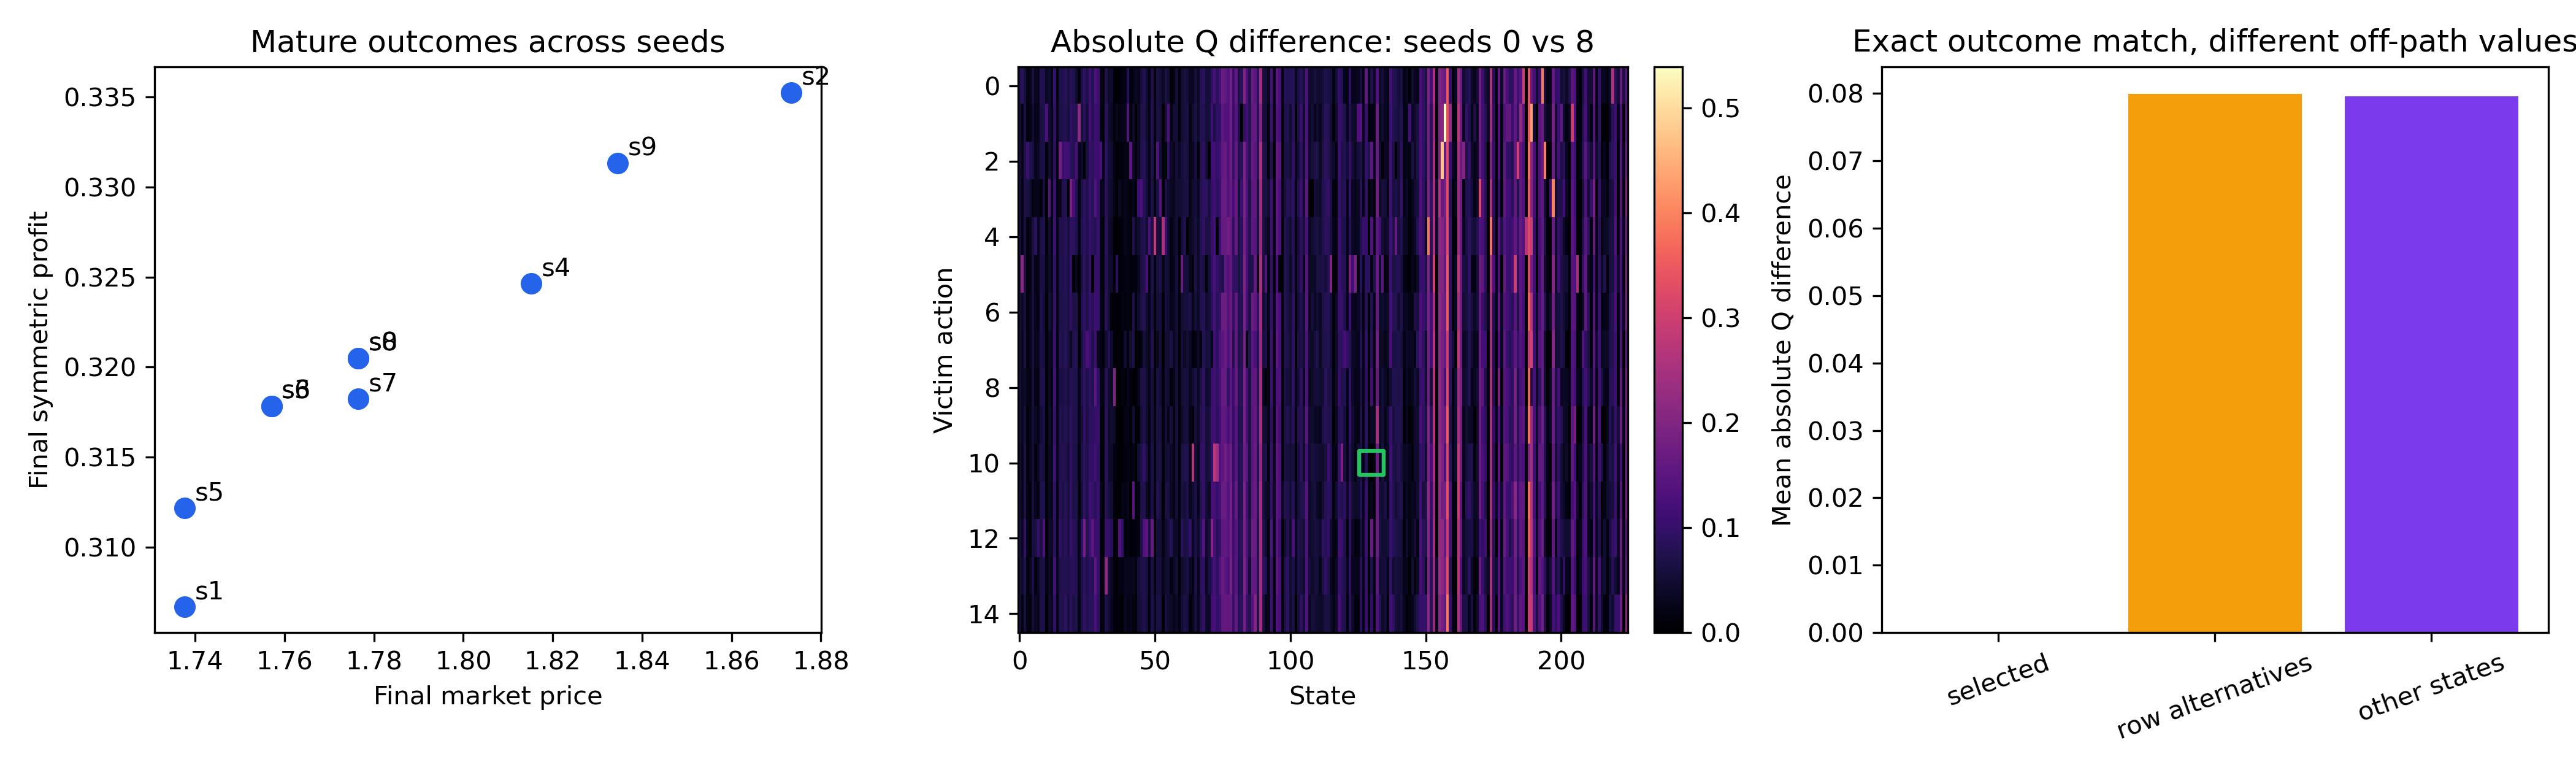
\includegraphics[width=\textwidth]
{../analysis/mature_qtable_heterogeneity/mature_qtable_heterogeneity.png}
\caption{Mature Q-vs-Q outcomes and off-path Q-table heterogeneity. The
seed-0/seed-8 comparison holds the terminal outcome fixed while revealing
different values away from the recurrent path.}
\label{fig:qtable}
\end{figure}

A local Q-gap clarifies why permission to update need not produce an immediate
policy switch. If \(a^*\) is currently greedy at \(s^*\), define
\[
\Delta Q_t(s^*,a^*)=
Q_t(s^*,a^*)-\max_{a\ne a^*}Q_t(s^*,a).
\]
A one-step sufficient condition for the selected action to remain greedy is
\[
\alpha |TD_t|<\Delta Q_t(s^*,a^*).
\]
This inequality is a local diagnostic, not a collusion theorem. It explains
how a live-update-permitted mature learner can remain behaviorally stable over
short windows while still differing conceptually from a frozen policy.

\section{Discussion and Limitations}

The two results concern different parts of the same identification problem.
RQ1 shows that the opponent's update rule is part of the evaluation estimand.
RQ2 shows that, along the tested information ladder, neither richer
representation nor escalating access to incumbent information recreates the
mature Q-vs-Q convention.
Descriptively, the failures differ: full-information regret matching settles
into a stable low-price regime,
some opponent-aware runs provide a price umbrella to the incumbent, and
representation objectives improve internal prediction without restoring the
high-price outcome. These labels summarize observed trajectories; they are not
learner-level causal effects.

The evidence covers one Bertrand-logit calibration, one action grid, finite
training budgets, and a tabular Q-learning incumbent. The RQ1 full-design
contrast combines maturity with freezing, whereas its paired evaluation
isolates update permission over a finite continuation window. Learner
configurations differ in horizon and information set, so we report
recoverability rather than a ranking. Welfare is intramodel log-bin accounting,
not an identified policy effect.

\section{Conclusion}

Fixed-opponent evaluation and live-update continuation are different empirical
objects. In this pricing game, DQN performance against a frozen mature
Q-learner is checkpoint-specific and changes when incumbent updates are
permitted. Across the tested information ladder, no configuration recovers the mature
Q-vs-Q high-price convention. Evaluation protocol and
information access should therefore be reported as part of the result.

\appendix

\section{Architecture Specifications}
\label{app:architectures}

\begin{figure}[H]
\centering
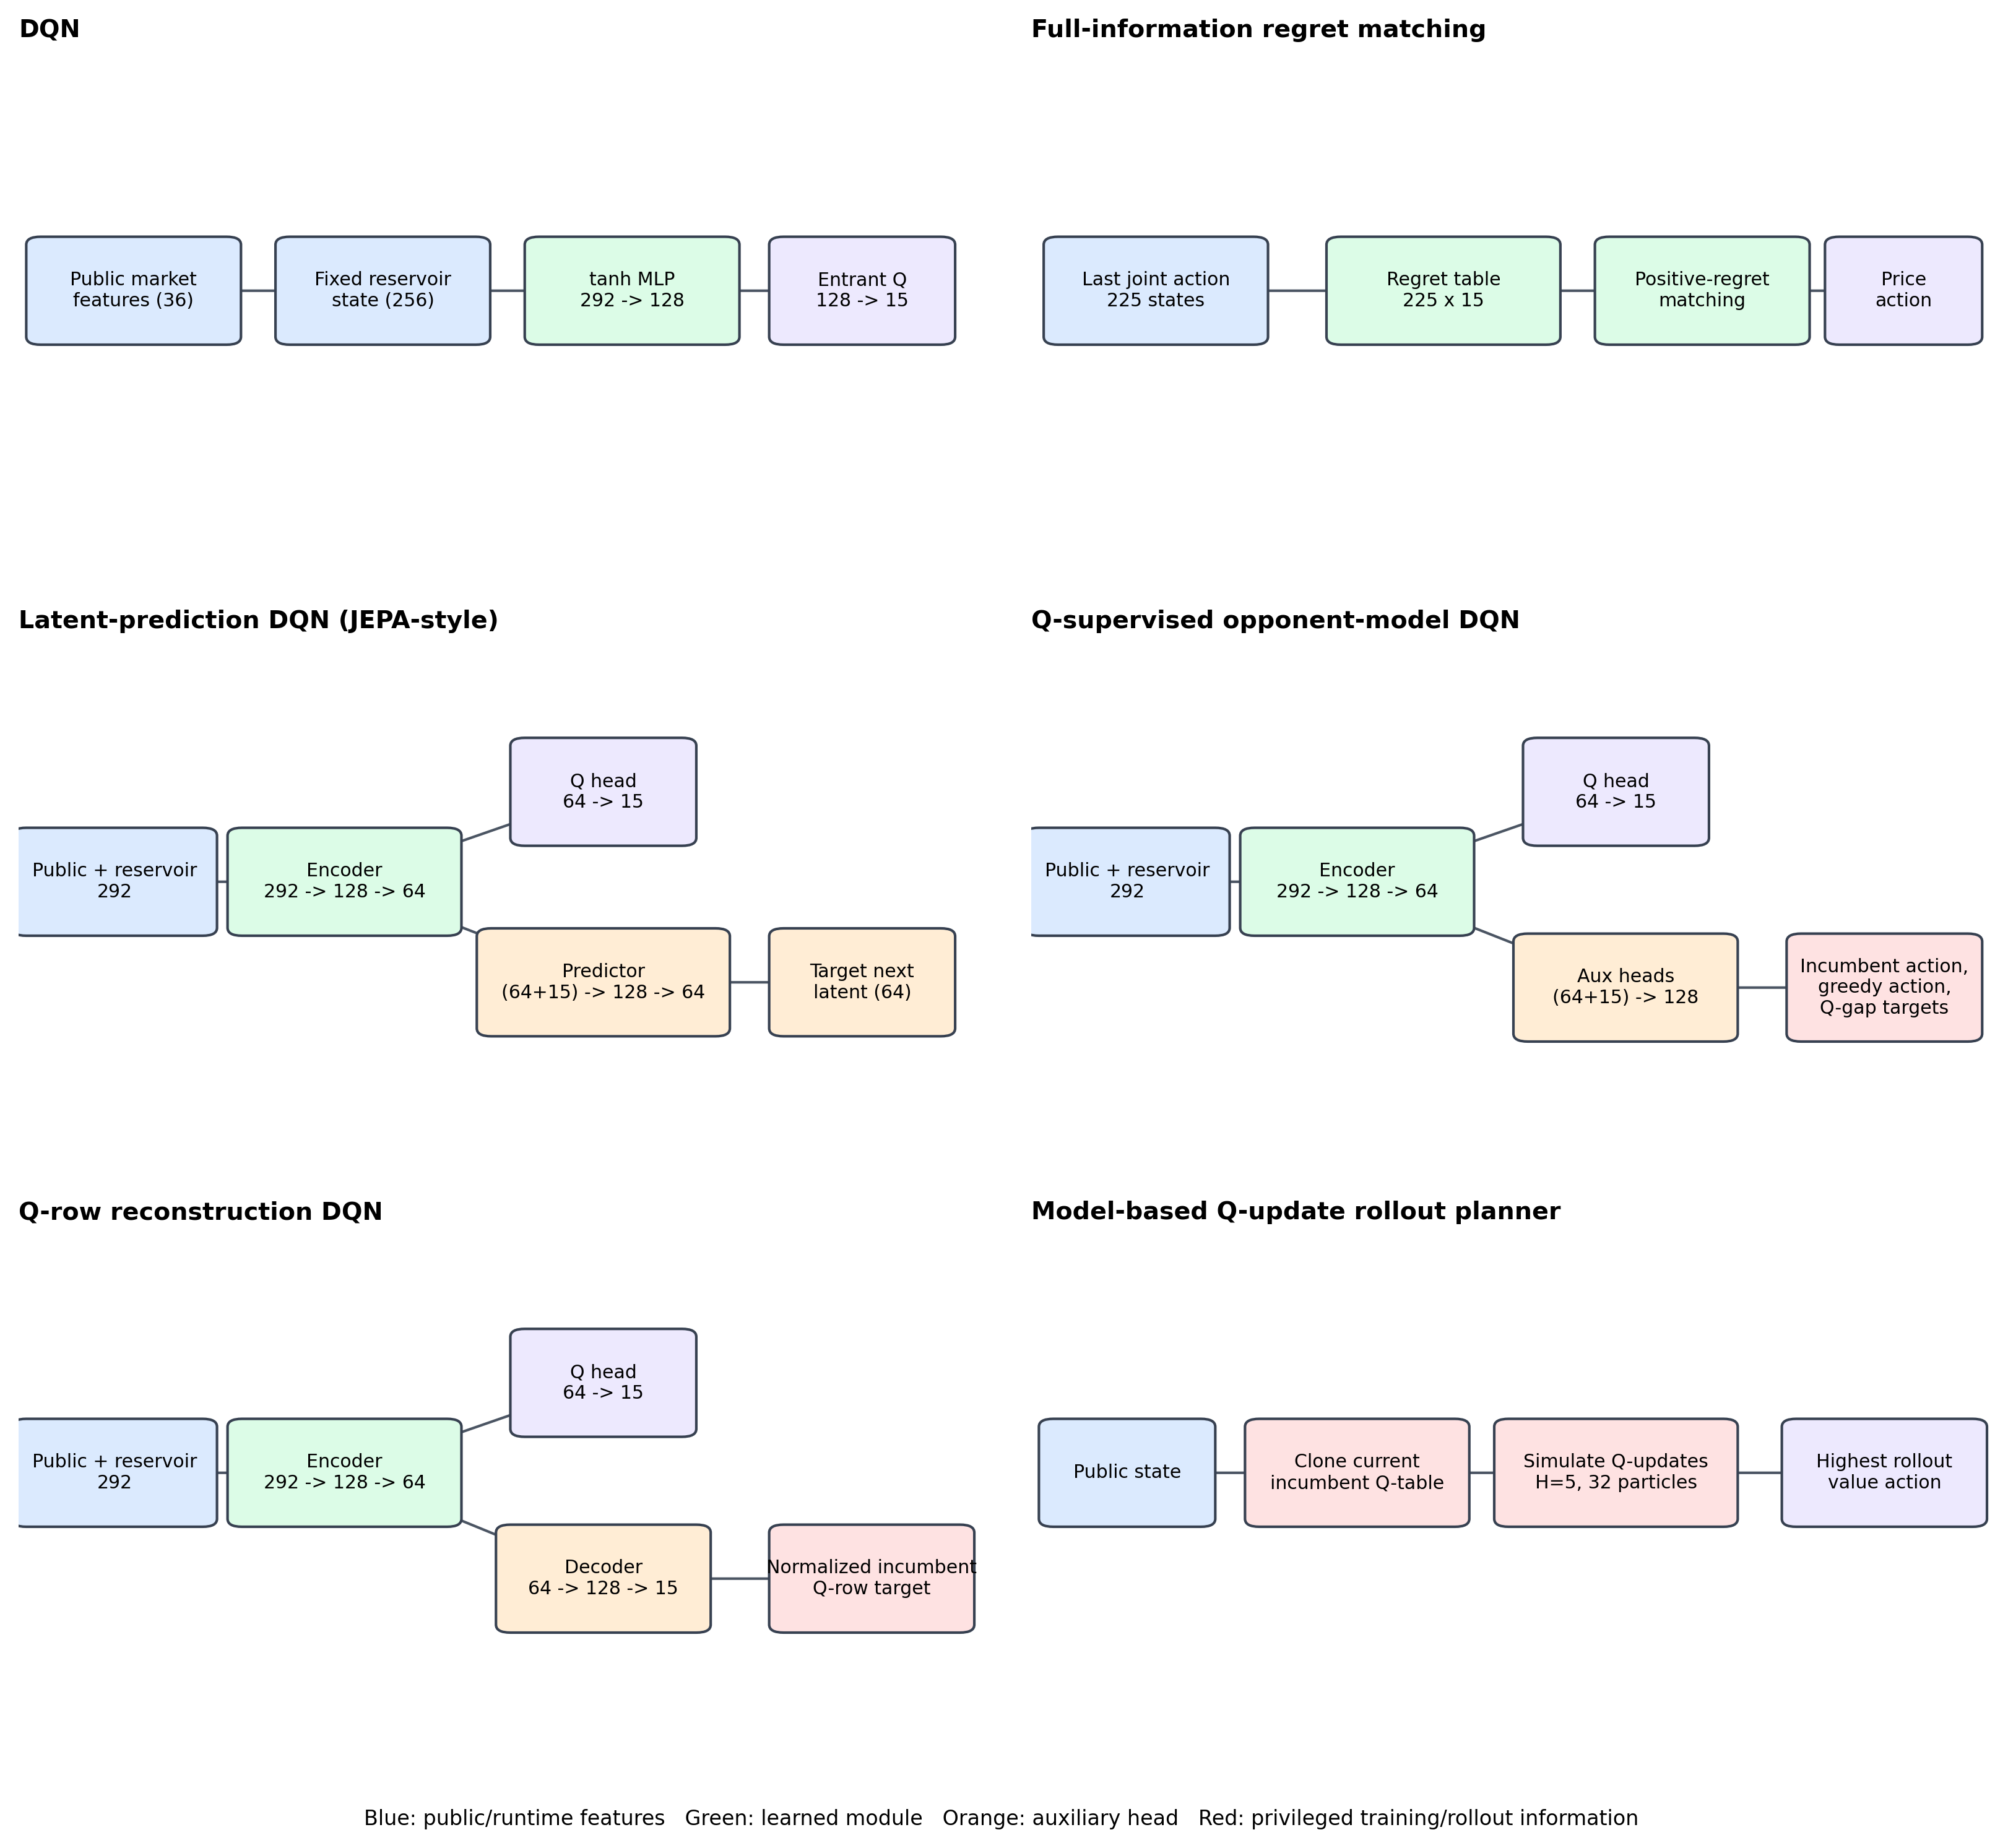
\includegraphics[width=\textwidth]{../paper_figures/architecture_overview.png}
\caption{Implemented learner and information flows. Red elements denote
incumbent-Q or incumbent-update information unavailable to public-history-only
learners.}
\end{figure}

\paragraph{DQN.}
The public observation contains normalized price history, price changes, price
gap and mean, market shares, and margins. With \(H=8\), the public vector has
dimension 36. A fixed 256-dimensional reservoir is appended. The learned
network is \(292\to128\to15\), with a tanh hidden layer, Bellman squared-error
loss, replay capacity 100,000, and a target network.

\paragraph{Tabular full-information regret matching.}
The previous joint action indexes 225 information states. Each rollout replica
stores a \(225\times15\) cumulative-regret table. Positive regrets define the
mixed strategy. Updates use the one-period counterfactual entrant profit of
every action against the realized incumbent action.

\paragraph{Latent-prediction DQN (JEPA-style).}
A \(292\to128\to64\) encoder feeds a linear 15-action Q-head. An auxiliary
predictor maps the latent state and a one-hot entrant action,
\(79\to128\to64\), to the target network's next latent state. The objective is
TD loss plus \(0.1\) times latent-prediction loss.

\paragraph{Q-supervised opponent-model DQN.}
The policy path is \(292\to128\to64\to15\). Auxiliary heads predict realized
and greedy incumbent actions, anchor compliance, the anchor Q-gap, and market
features. Runtime actions use public features, but greedy-action and Q-gap
labels are read from the incumbent Q-table during training.

\paragraph{Q-row reconstruction DQN.}
A \(64\to128\to15\) decoder is added to the latent-prediction encoder and trained to
reconstruct a normalized row of the incumbent Q-table. It is a privileged
representation probe.

\paragraph{Model-based Q-update rollout planner.}
For every candidate action, the planner clones the incumbent table and
simulates epsilon-greedy incumbent actions and Q-updates for horizon five with
32 particles. It selects the action with the greatest simulated discounted
entrant profit.
Direct access to the table and update rule makes this a privileged
model-access probe.

\section{Statistical Results}
\label{app:statistics}

\begin{table}[H]
\centering
\caption{Seed-level own-profit comparisons with the mature Q-vs-Q
distribution.}
\scriptsize
\begin{tabular}{lrrrr}
\toprule
Learner & Difference & Bootstrap 95\% CI & Exact \(p\) & Holm \(p\) \\
\midrule
DQN & -0.032919 & [-0.041969, -0.024210] & \(1.08{\times}10^{-5}\) & \(6.50{\times}10^{-5}\) \\
Full-information regret matching & -0.052343 & [-0.057409, -0.047444] & \(1.08{\times}10^{-5}\) & \(6.50{\times}10^{-5}\) \\
Latent-prediction DQN & -0.028162 & [-0.033693, -0.022845] & \(1.08{\times}10^{-5}\) & \(6.50{\times}10^{-5}\) \\
Q-supervised opponent-model DQN & -0.031026 & [-0.038958, -0.023874] & \(1.08{\times}10^{-5}\) & \(6.50{\times}10^{-5}\) \\
Q-row reconstruction DQN & -0.040022 & [-0.056184, -0.028417] & \(1.08{\times}10^{-5}\) & \(6.50{\times}10^{-5}\) \\
Q-update rollout planner & -0.024559 & [-0.029605, -0.019657] & \(1.08{\times}10^{-5}\) & \(6.50{\times}10^{-5}\) \\
\bottomrule
\end{tabular}
\end{table}

\begin{table}[H]
\centering
\caption{Seed-level mean-market-price comparisons with the mature Q-vs-Q
distribution.}
\scriptsize
\begin{tabular}{lrrrr}
\toprule
Learner & Difference & Bootstrap 95\% CI & Exact \(p\) & Holm \(p\) \\
\midrule
DQN & -0.102099 & [-0.143546, -0.060071] & \(3.90{\times}10^{-4}\) & \(3.90{\times}10^{-4}\) \\
Full-information regret matching & -0.228735 & [-0.255939, -0.205311] & \(1.08{\times}10^{-5}\) & \(6.50{\times}10^{-5}\) \\
Latent-prediction DQN & -0.189064 & [-0.221684, -0.159152] & \(1.08{\times}10^{-5}\) & \(6.50{\times}10^{-5}\) \\
Q-supervised opponent-model DQN & -0.149740 & [-0.185416, -0.113893] & \(1.08{\times}10^{-5}\) & \(6.50{\times}10^{-5}\) \\
Q-row reconstruction DQN & -0.141354 & [-0.187182, -0.095569] & \(8.66{\times}10^{-5}\) & \(1.73{\times}10^{-4}\) \\
Q-update rollout planner & -0.119066 & [-0.146290, -0.095564] & \(1.08{\times}10^{-5}\) & \(6.50{\times}10^{-5}\) \\
\bottomrule
\end{tabular}
\end{table}

Each difference is the learner mean minus the mean across ten independent
mature Q-vs-Q checkpoints. Exact tests enumerate assignments of the 20
seed-level observations and test equality of distributions under
exchangeability, rather than equality of means alone. Percentile bootstrap
intervals use 10,000 resamples of both groups. Holm adjustment covers all six
configurations separately within the profit and mean-price families. Because
the same mature reference is reused, the six contrasts are dependent; the
reported intervals are marginal, not simultaneous.

\section{Static Benchmarks}

At a symmetric price \(p\), the Nash first-order condition is
\[
1-\frac{p-c}{\mu}(1-\rho_i(p,p))=0.
\]
For a common-price joint-profit choice, with outside share
\(\rho_0(p,p)=1-2\rho_i(p,p)\), the first-order condition is
\[
1-\frac{p-c}{\mu}\rho_0(p,p)=0.
\]
Numerical solutions give the grid anchors reported in Section 3.

\section{Q-Table Projection}

\begin{figure}[H]
\centering
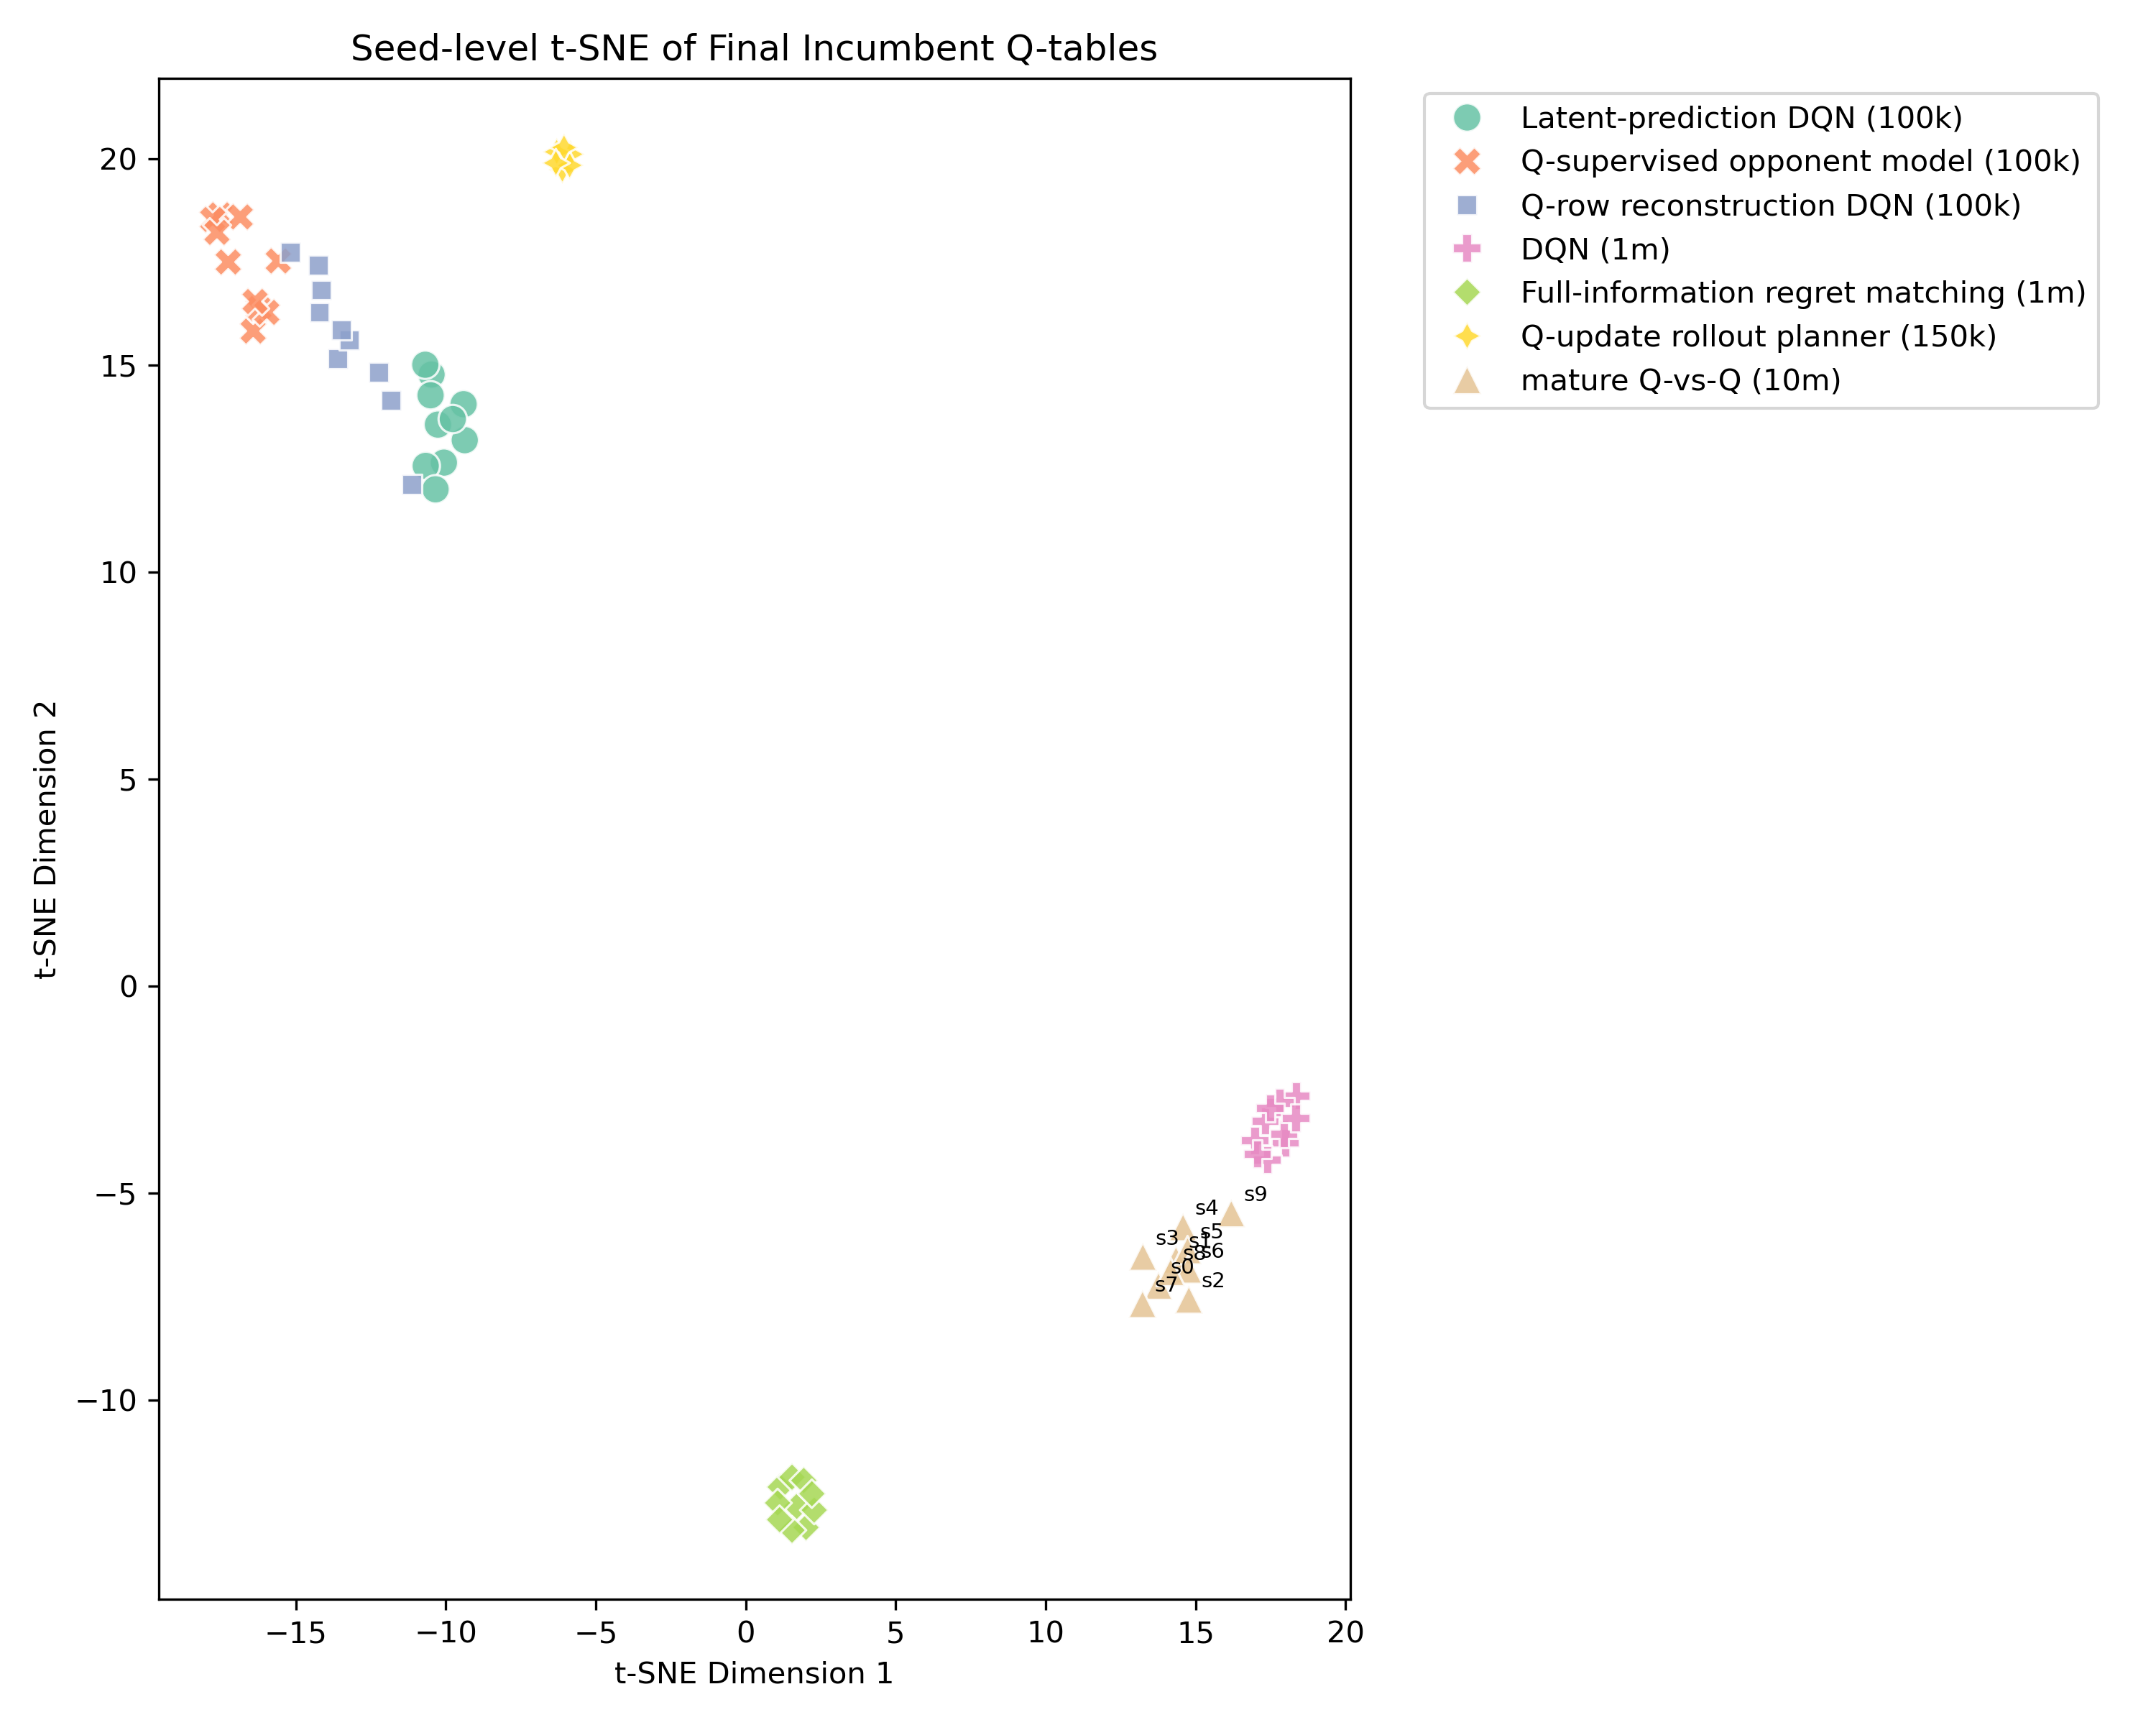
\includegraphics[width=0.9\textwidth]{../paper_figures/tsne_victim_qtables.png}
\caption{Seed-level t-SNE projection of final incumbent Q-tables. Independent
mature Q-vs-Q seeds occupy different locations, and different learner
architectures lead to different final incumbent-table regions. The
latent-prediction, Q-supervised opponent-model, and Q-row reconstruction DQNs
occupy neighboring or partially overlapping regions. The projection is
descriptive and not inferential evidence.}
\end{figure}

\clearpage
\section{Claim Ledger}

\begin{table}[H]
\centering
\small
\begin{tabularx}{\textwidth}{L{0.27\textwidth}YY}
\toprule
Claim & Evidence & Boundary \\
\midrule
Frozen and live-update continuation estimate different objects. &
Ten mature checkpoints, three DQN seeds each, with matched frozen and
live-update-permitted evaluation. &
Finite post-training continuation; update permission does not imply a
greedy-policy switch. \\

Frozen-mature entrant performance is checkpoint-specific. &
Checkpoint-level distribution and full-design comparison with registered
joint learning. &
The full-design contrast combines maturity and freezing. \\

Public-information configurations remain below mature Q-vs-Q. &
Seed-level profit and mean-price tests for DQN, regret matching,
latent-prediction, and Q-supervised opponent-model learners. &
One market and unequal horizons; a recoverability test, not a ranking. \\

Privileged probes at the top of the ladder also remain below. &
Q-row reconstruction and Q-update rollout diagnostics. &
Highest information rung; recovery still absent at unequal horizons. \\

Log-bin consumer surplus is higher relative to mature Q-vs-Q. &
Last-100k weighted training bins; positive CS differences for all reported rows. &
\(CS(E[p\mid b])\) approximation; total-welfare evidence varies by learner. \\
\bottomrule
\end{tabularx}
\end{table}

\section{Reproducibility}

All manuscript numbers are generated from seed-level result artifacts and the
experiment registry. The reproduction scripts construct the reference
distribution, statistical tables, log-bin welfare approximation, figures, and
protocol contrasts. Raw result files are not edited during manuscript
generation. Replication code and seed-level data are available at
\url{https://github.com/danilamalafeev/algorithmic-pricing-continuation}.

\footnotesize
\begin{thebibliography}{9}

\bibitem{calvano2020}
Calvano, E., Calzolari, G., Denicolo, V., and Pastorello, S. (2020).
Artificial intelligence, algorithmic pricing, and collusion.
\emph{American Economic Review}, 110(10):3267--3297.

\bibitem{abada2024}
Abada, I., Lambin, X., and Tchakarov, N. (2024).
Collusion by mistake: Does algorithmic sophistication drive
supra-competitive profits?
\emph{European Journal of Operational Research}, 319:927--940.

\bibitem{shidideng2025}
Deng, S., Schiffer, M., and Bichler, M. (2025).
Exploring competitive and collusive behaviors in algorithmic pricing with
deep reinforcement learning.
arXiv:2503.11270.

\bibitem{aideng2026}
Deng, A. (2026).
Algorithmic collusion or algorithmic confusion? Rethinking the risks of AI
pricing for companies and policymakers.
SSRN working paper 6823199, draft dated May 24, 2026.

\bibitem{carissimo2025}
Carissimo, C., Falniowski, F., Rahimi, S., and Nax, H. (2025).
Algorithmic collusion is algorithm orchestration.
arXiv:2508.14766.

\bibitem{hernandez2017}
Hernandez-Leal, P., Kaisers, M., Baarslag, T., and de Cote, E. M. (2017).
A survey of learning in multiagent environments: Dealing with
non-stationarity.
arXiv:1707.09183.

\bibitem{papoudakis2019}
Papoudakis, G., Christianos, F., Schafer, L., and Albrecht, S. V. (2019).
Dealing with non-stationarity in multi-agent deep reinforcement learning.
arXiv:1906.04737.

\bibitem{foerster2018}
Foerster, J., Chen, R. Y., Al-Shedivat, M., Whiteson, S., Abbeel, P., and
Mordatch, I. (2018).
Learning with opponent-learning awareness.
\emph{Proceedings of AAMAS}.

\bibitem{fung2024}
Fung, K., Zhang, Q., Lu, C., Wan, J., Willi, T., and Foerster, J. (2024).
Analysing the sample complexity of opponent shaping.
\emph{Proceedings of AAMAS}.

\end{thebibliography}
\normalsize

\end{document}
